\documentclass[final,5p,times,twocolumn]{elsarticle}

\usepackage{amsmath}
\usepackage{amssymb}
\usepackage{graphicx}
\usepackage{booktabs}
\usepackage{placeins}
\usepackage{algorithm}
\usepackage{algorithmic}
\usepackage{subcaption}
\usepackage{xcolor}
\usepackage{hyperref}
\hypersetup{hidelinks}
\usepackage{multirow}
\usepackage{siunitx}
\usepackage{array}
\setlength{\emergencystretch}{1em}
\makeatletter
\setlength{\@dblfptop}{0pt}
\setlength{\@dblfpsep}{14pt}
\setlength{\@dblfpbot}{0pt plus 1fil}
\makeatother

\journal{Electric Power Systems Research}
\biboptions{sort&compress}

\newcommand{\R}{\mathbb{R}}
\newcommand{\C}{\mathbb{C}}
\newcommand{\Nset}{\mathcal{N}}
\newcommand{\Lset}{\mathcal{L}}
\newcommand{\Bset}{\mathcal{B}}
\newcommand{\Xset}{\mathcal{X}}
\newcommand{\Gset}{\mathcal{G}}
\newcommand{\Tset}{\mathcal{T}}
\newcommand{\relu}{\operatorname{ReLU}}
\newcommand{\diag}{\operatorname{diag}}
\newcommand{\mean}{\operatorname{mean}}
\newcommand{\vect}{\operatorname{vec}}
\newcommand{\given}{\,\middle|\,}

\begin{document}
\raggedbottom

\begin{frontmatter}

\title{GFNO-PINO: A Topology-Disjoint Benchmark Isolating Physics
Fine-Tuning, Topology Conditioning, and Spectral Filtering in AC-OPF Graph
Surrogates}

\author[inst1]{Roshan Kumar Sharma}
\author[inst1]{Ujjwal Prasad Dahal}

\affiliation[inst1]{
  organization={Department of Electrical Engineering, Purwanchal Campus,
  Institute of Engineering, Tribhuvan University},
  city={Dharan},
  country={Nepal}
}

\begin{abstract}
Security assessment requires repeated alternating-current optimal power-flow
(AC-OPF) solutions as injections and line availability change. Although
topology inputs and spectral graph filters are architecturally plausible for
this task, their benefit relative to physics-informed fine-tuning has not been
isolated under matched, topology-disjoint comparisons. To test these choices,
we construct a topology-conditioned Chebyshev graph surrogate (GFNO-PINO) that
maps nodal injections, directional branch admittances, line status, equipment
limits, and generator economics to voltage phasors and dispatch. It combines a
supervised PowerModels--IPOPT warm start with exact differentiable AC
residuals and zero-safe gradient-norm balancing; independent voltage and
generator boxes and the reference angle are enforced by construction, while
coupled AC constraints remain soft. The five-seed pilot benchmark covers IEEE
30-, 57-, 118-, and 300-bus cases, three unseen line-outage topologies per
case, and five neural models. Relative to the data-only GFNO, paired physics
fine-tuning reduces mean sample-maximum power-balance mismatch by
63.4--89.3\%, and all 20 paired seed effects are positive; the accompanying
seed-resampling intervals are descriptive, not population-confidence claims.
In contrast, the parameter-matched topology-blind GFNO and spatial GNN match
or outperform GFNO-PINO on three of four systems, so this benchmark does not
establish a causal accuracy benefit from either explicit topology input or
Chebyshev filtering. Every learned model obtains 0\% feasibility under the
declared proxy; GFNO-PINO's mean maximum mismatch remains 0.281, 1.684, 0.890,
and 5.959 p.u. from 30 to 300 buses. GPU forward-pass medians yield raw
device-specific latency ratios of 8.3--138.1$\times$ relative to stored IPOPT
CPU solve medians, excluding verification and restoration. The contribution
is therefore a controlled ablation identifying physics fine-tuning as the
validated driver under this protocol and documenting unconfirmed
architectural hypotheses, not a production-ready or exactly feasible solver.
\end{abstract}

\begin{keyword}
AC-OPF \sep Physics-Informed Learning \sep N-1 Contingency
\sep Chebyshev Graph Neural Network \sep Renewable Integration
\end{keyword}

\end{frontmatter}

\section{Introduction}
\label{sec:introduction}

Power-system operation is being reshaped by variable renewable generation,
electrification, and increasingly active demand. Solar and wind injections can
change substantially within an operating interval, while load uncertainty
alters both active- and reactive-power requirements. At the same time, the
N-1 security criterion requires operators to assess whether the system remains
within voltage, generation, and branch-flow limits after the loss of any
credible component. These interacting sources of variability turn dispatch
into a sequence of closely spaced, nonlinear, topology-dependent optimization
problems rather than a single deterministic calculation. Reviews of optimal
power flow (OPF) and security-constrained OPF emphasize both their operational
importance and their continuing computational difficulty
\cite{frank2016opf,capitanescu2016critical,molzahn2019survey,zohrizadeh2020conic}.

The alternating-current OPF (AC-OPF) formulation represents voltage magnitudes,
phase angles, active and reactive generation, losses, transformer effects, and
thermal constraints. This fidelity produces non-convex equality and inequality
constraints. Mature nonlinear solvers such as IPOPT apply sparse primal-dual
interior-point methods and are indispensable for offline planning and
high-quality reference solutions \cite{wachter2006ipopt}. Nevertheless, a
complete solve is still required for each loading condition and each network
topology. Under large scenario ensembles or online contingency screening,
solver initialization, factorization, and convergence variability can become a
latency bottleneck. Convex relaxations can provide valuable bounds but introduce
their own tightness and scalability tradeoffs \cite{zohrizadeh2020conic}.

The direct-current OPF (DC-OPF) approximation is faster because it neglects
reactive power, assumes voltage magnitudes near one per unit, and linearizes
angle differences. These assumptions make DC-OPF useful for screening and
market studies, but they can produce material errors under high loading,
resistive networks, voltage-sensitive conditions, or binding reactive-power
limits, as documented in \cite{stott2009dc}. A real-time AC-OPF surrogate should be
benchmarked against DC-OPF for speed without treating the linear approximation
as an AC-feasible reference.

Learning-based OPF methods amortize the cost of optimization: an expensive
solver generates training examples offline, after which a neural network
provides rapid online predictions. DeepOPF and related methods demonstrate the
potential of predict-and-reconstruct strategies, feasibility-aware training,
and topology embeddings
\cite{pan2021deepopf,pan2023acdeepopf,zhou2023deepopfft}.
Other work combines supervised learning with Lagrangian penalties or
worst-case verification \cite{fioretto2020predicting,venzke2020worstcase}.
However, a finite-dimensional network trained on one fixed ordering can learn
spurious correlations specific to that network. Even when admittance is an
input, dense architectures do not directly encode the locality, permutation
structure, or graph spectrum of an electrical network.

Physics-informed neural networks (PINNs) reduce reliance on labels by penalizing
governing-equation residuals \cite{raissi2019pinn,karniadakis2021piml}. In power
systems, PINNs have been used to embed power-flow or optimality equations
\cite{misyris2020pinn,nellikkath2022acopf,lei2021datadriven}. A standard PINN
nevertheless represents a solution for a fixed physical instance or uses a
fixed-dimensional parameterization. If its residual is formed with one
admittance matrix, replacing a line changes the governing operator itself.
Retraining a separate PINN for each contingency defeats the intended real-time
advantage.

Neural operators provide a more suitable abstraction: they learn maps between
function spaces rather than a single input-output vector relationship.
DeepONet learns an operator through branch and trunk networks
\cite{lu2021deeponet}, while the Fourier neural operator (FNO) parameterizes
non-local integral kernels in a spectral domain \cite{li2021fno,kova2023neuralop}.
The original FNO assumes a regular Euclidean grid and a shared Fourier basis,
whereas transmission networks are sparse, irregular graphs. Graph spectral
methods replace Euclidean harmonics with functions of the graph Laplacian
\cite{hammond2011wavelets,defferrard2016chebnet,bronstein2017geometric}.
Chebyshev polynomial filters are particularly attractive under contingencies:
they apply the same learned spectral multiplier to a changing Laplacian without
requiring a topology-specific eigendecomposition or eigenvector alignment.

This paper conducts a controlled, topology-disjoint ablation of physics
fine-tuning, explicit topology conditioning, and Chebyshev spectral filtering
for AC-OPF graph surrogates. GFNO-PINO is the experimental instrument for
separating these effects, not a presupposed superior architecture. The
principal contributions are:

\begin{itemize}
  \item A differentiable AC physics objective using exact bus-admittance and
  branch-current operators, coupled with adaptive gradient-norm loss balancing
  and a supervised-to-physics curriculum. Hard transformations enforce
  independent voltage and generator boxes and the slack reference, while all
  coupled constraints that remain approximate are reported.
  \item A reproducible five-seed, topology-disjoint pilot benchmark on four IEEE
  systems against IPOPT AC-OPF, DC-OPF, a base-only PINN, a parameter-matched
  topology-blind GFNO, a spatial GNN, and a data-only graph FNO.
  \item A topology-conditioned graph-surrogate formulation, evaluated as a
  hypothesis under test, in which directional admittance, status, and rating
  alter both the learned propagation graph and the sample-specific AC residual.
  \item The validated empirical finding that paired physics fine-tuning reduces
  mean sample-maximum balance mismatch by 63.4--89.3\% relative to data-only
  training under this pilot protocol, with all 20 paired seed effects positive.
  \item The negative empirical finding that explicit topology conditioning and
  Chebyshev filtering do not establish a causal accuracy benefit: matched
  topology-blind and spatial baselines match or outperform the full model on
  three of four systems. Every learned model remains 0\% feasible under the
  declared proxy.
\end{itemize}

Reporting the unfavorable architectural ablations is part of the contribution:
it distinguishes the validated effect (physics fine-tuning) from the
unconfirmed effects (topology conditioning and spectral filtering) and informs
which surrogate-design complexity is justified by the present evidence.

The remainder of the paper is organized as follows. Section~\ref{sec:related}
reviews classical, learning-based, physics-informed, and neural-operator
approaches. Section~\ref{sec:methodology} presents the AC-OPF formulation and
the benchmarked GFNO-PINO architecture. Section~\ref{sec:experiments} defines the benchmark
protocol. Section~\ref{sec:results} reports and discusses the executed
benchmark.
Section~\ref{sec:limitations} states the scope of the feasibility and
generalization claims, and Section~\ref{sec:conclusion} concludes the paper.

\section{Related work}
\label{sec:related}

\subsection{Classical and learning-based AC-OPF}

AC-OPF is a foundational nonlinear optimization problem in power-system
planning and operation. Standard formulations minimize generation cost subject
to nonlinear nodal balances and equipment constraints
\cite{frank2016opf,capitanescu2016critical}. Sparse interior-point algorithms
provide reliable local solutions and form the basis of widely used tools
\cite{wachter2006ipopt}. MATPOWER, pandapower, and PowerModels provide
reproducible implementations and test-case interfaces
\cite{zimmerman2011matpower,thurner2018pandapower,coffrin2018powermodels}.
Because AC-OPF is non-convex, a locally converged point is not in general a
certificate of global optimality. Convex and moment relaxations may produce
bounds or exact solutions in favorable cases, but no single relaxation
dominates across all large practical networks \cite{molzahn2019survey,
zohrizadeh2020conic}.

Supervised surrogates learn the mapping from uncertain demand to optimal
decisions. DeepOPF predicts independent variables and reconstructs dependent
quantities to improve feasibility \cite{pan2021deepopf,pan2023acdeepopf}.
Fioretto et al.\ combine deep learning with a Lagrangian-dual objective
\cite{fioretto2020predicting}; Venzke et al.\ formulate optimization problems
that bound worst-case neural-network violations
\cite{venzke2020worstcase}. These approaches show that inference can be much
faster than solving each instance from scratch, but feasibility treatment and
generalization domains differ. DeepOPF-FT is especially relevant because it
embeds topology and admittance to address multiple related AC-OPF problems
\cite{zhou2023deepopfft}. The present work differs by using graph-spectral
propagation that changes with the input topology and by training with exact AC
residuals.

\subsection{Physics-informed neural networks in power systems}

PINNs augment data losses with residuals of governing equations
\cite{raissi2019pinn}. The broader physics-informed machine-learning framework
can improve data efficiency and physical consistency, but optimization can be
stiff when residual terms have different units or gradient scales
\cite{karniadakis2021piml}. In power applications, Misyris et al.\ embedded
power-system equations in neural training \cite{misyris2020pinn}, and Lei
et al.\ developed a physics-informed data-driven OPF framework
\cite{lei2021datadriven}. Nellikkath and Chatzivasileiadis incorporated AC-OPF
physics and methods for reducing worst-case violations
\cite{nellikkath2022acopf}.

Physics penalties do not automatically provide feasibility. A small mean
residual can coexist with a large worst-bus error, and weighted penalties may
trade economic performance against constraint satisfaction. Furthermore, a
PINN residual evaluated using one fixed $Y_{\mathrm{bus}}$ does not describe
the equations after a branch outage. The network may be fine-tuned for every
new $Y_{\mathrm{bus}}$, but such a workflow is not topology independent.
The topology-conditioned formulation under test instead treats topology as
part of the input function and evaluates every residual with the corresponding
sample-specific admittance operators.

\subsection{Neural operators and graph spectral methods}

DeepONet establishes a practical architecture for learning nonlinear operators
using separate encoders for input functions and output coordinates
\cite{lu2021deeponet}. FNO learns a global convolution kernel in Fourier space
and has demonstrated mesh-transfer properties for parametric partial
differential equations \cite{li2021fno}. Neural-operator theory formalizes
discretization-aware mappings between infinite-dimensional spaces
\cite{kova2023neuralop}. Applying a Euclidean FFT directly to buses, however,
would assign physical meaning to an arbitrary bus ordering and would not
respect irregular connectivity.

Graph signal processing defines spectral filters through the eigenstructure of
the graph Laplacian \cite{hammond2011wavelets}. Chebyshev networks approximate
such filters by stable polynomials, avoiding explicit eigendecomposition
\cite{defferrard2016chebnet}. Graph convolution and geometric deep learning
extend local and spectral operations to non-Euclidean domains
\cite{kipf2017gcn,bronstein2017geometric}. In power systems, graph neural
solvers exploit network structure for power flow and OPF
\cite{donon2019graphsolver,owerko2020opfgnn}. A spatial GNN aggregates nearby
features, whereas a polynomial spectral filter parameterizes a frequency
response of the topology-conditioned Laplacian. However, the implemented
Chebyshev layer has the same localized polynomial form as ChebNet. Because
this study trains a separate checkpoint per system size and performs no
mesh-refinement or discretization-transfer experiment, it does not claim the
stronger function-space generalization normally associated with neural
operators. ``GFNO-PINO'' is retained as the implementation name, not as
evidence of such a property.

\subsection{Research gap}

The preceding literatures leave a specific gap. Classical methods account for
topology and AC physics but solve every scenario separately. Supervised OPF
surrogates provide low latency but can be tied to a fixed dimension and may
require post-processing. PINNs inject physics but are commonly trained for a
fixed admittance matrix. Neural operators target families of equations, yet
standard FNOs assume a regular grid, and existing OPF GNNs do not necessarily
combine graph-spectral propagation, sample-specific AC residuals, adaptive
multi-objective training, and topology-disjoint evaluation. This work addresses
that intersection. ``Topology conditioned'' means that one parameter set
processes the base grid and unseen non-islanding line-status configurations
within a fixed test-system family; it does not imply universal zero-shot
transfer to arbitrary utilities, generator sets, or unbounded network sizes.
Whether this input actually improves accuracy relative to simpler
architectures is treated as an empirical question and tested directly in
Section~\ref{subsec:ablation}, where it is not confirmed under the present
protocol.

\section{Methodology}
\label{sec:methodology}

\subsection{AC-OPF problem formulation}
\label{subsec:acopf}

Let $\Nset$, $\Lset$, $\Xset$, $\Bset=\Lset\cup\Xset$, and $\Gset$ denote the
bus, physical-line, fixed-transformer, full canonical-branch, and
dispatchable-generator sets, respectively. Each branch $a\in\Bset$ has one
canonical from/to orientation and two terminal equations. The physical-line
status vector is $z\in\{0,1\}^{|\Lset|}$, and its full-branch status map is
\begin{equation}
  s_a(z)=
  \begin{cases}
    z_a, & a\in\Lset,\\
    1, & a\in\Xset.
  \end{cases}
  \label{eq:full_branch_status}
\end{equation}
Thus transformers participate in every graph and AC operator but are not
outage candidates in this benchmark.
Generator-to-bus incidence is represented by
$\Gset_i\subseteq\Gset$. For bus $i$, the voltage phasor is
$\mathcal{V}_i=V_i e^{\mathrm{j}\theta_i}$. Active and reactive demand are
$P_i^d,Q_i^d$, renewable active injection is $P_i^r$, and dispatchable
generation is $P_g^g,Q_g^g$. With quadratic cost coefficients
$c_{2g},c_{1g},c_{0g}$, AC-OPF is
\begin{align}
  \underset{\substack{V,\theta,P^g,Q^g}}{\operatorname{minimize}}
  \quad
  C(P^g)
  &=
  \sum_{g\in\Gset}
  \left(c_{2g}(P_g^g)^2+c_{1g}P_g^g+c_{0g}\right).
  \label{eq:objective}
\end{align}

For topology $z$, let
$Y(z)=G(z)+\mathrm{j}B(z)\in\C^{|\Nset|\times|\Nset|}$ be the bus-admittance
matrix. A base topology has $z_\ell=1$ for every in-service line. An N-1
topology sets exactly one eligible physical-line status to zero. With
$z_k^{(\ell)}=1-\mathbb{I}[k=\ell]$, define the active full branch set
$\Bset(z)=\{a\in\Bset:s_a(z)=1\}$. The evaluated set is
\begin{equation}
  \Tset_{\mathrm{N-1}}
  =
  \left\{
    z^{(\ell)}
    \,\middle|\,
    \ell\in\Lset_{\mathrm{eligible}},\
    \left(\Nset,\Bset(z^{(\ell)})\right)\ {\rm connected}
  \right\}.
  \label{eq:nminusone}
\end{equation}
The active- and reactive-power injections implied by the voltage are
\begin{align}
  P_i(V,\theta;z)
  &=
  V_i\sum_{j\in\Nset}V_j
  \left[
    G_{ij}(z)\cos(\theta_i-\theta_j)
    +B_{ij}(z)\sin(\theta_i-\theta_j)
  \right],
  \label{eq:p_injection}\\
  Q_i(V,\theta;z)
  &=
  V_i\sum_{j\in\Nset}V_j
  \left[
    G_{ij}(z)\sin(\theta_i-\theta_j)
    -B_{ij}(z)\cos(\theta_i-\theta_j)
  \right].
  \label{eq:q_injection}
\end{align}
Kirchhoff's current law, written as nodal complex-power balance, requires
\begin{align}
  \sum_{g\in\Gset_i}P_g^g + P_i^r-P_i^d
  &=P_i(V,\theta;z),
  &&\forall i\in\Nset,
  \label{eq:p_balance}\\
  \sum_{g\in\Gset_i}Q_g^g-Q_i^d
  &=Q_i(V,\theta;z),
  &&\forall i\in\Nset.
  \label{eq:q_balance}
\end{align}
Equations~\eqref{eq:p_injection}--\eqref{eq:q_balance} are implemented in
complex form as
\begin{equation}
  S^{\mathrm{net}}
  =
  \mathcal{V}\odot\left(Y(z)\mathcal{V}\right)^*,
  \label{eq:complex_power}
\end{equation}
which is algebraically equivalent and avoids materializing a dense tensor of
all angle differences.

Let $Y_f(z)$ and $Y_t(z)$ map bus voltages to branch currents at the from and
to terminals. This representation retains line charging, off-nominal
transformer ratios, and phase shifts. Terminal powers are
\begin{align}
  S_a^f
  &=
  \mathcal{V}_{f(a)}
  \left([Y_f(z)\mathcal{V}]_a\right)^*,
  \label{eq:from_flow}\\
  S_a^t
  &=
  \mathcal{V}_{t(a)}
  \left([Y_t(z)\mathcal{V}]_a\right)^*,
  \label{eq:to_flow}
\end{align}
for $a\in\Bset$ with $s_a(z)=1$.
The remaining operating constraints are
\begin{align}
  P_g^{\min}\leq P_g^g\leq P_g^{\max},
  \quad
  Q_g^{\min}\leq Q_g^g\leq Q_g^{\max},
  &&\forall g\in\Gset,
  \label{eq:gen_limits}\\
  V_i^{\min}\leq V_i\leq V_i^{\max},
  &&\forall i\in\Nset,
  \label{eq:voltage_limits}\\
  \max\{|S_a^f|,|S_a^t|\}\leq S_a^{\max},
  &&\forall a\in\Bset:s_a(z)=1,
  \label{eq:thermal_limits}\\
  \underline{\Delta\theta}_a
  \leq \theta_{f(a)}-\theta_{t(a)}
  \leq \overline{\Delta\theta}_a,
  &&\forall a\in\Bset:s_a(z)=1,
  \label{eq:angle_limits}\\
  \theta_{i_{\mathrm{ref}}}=0.
  \label{eq:slack}
\end{align}
A zero MATPOWER branch rating denotes an unconstrained line and is excluded
from the thermal-violation denominator rather than interpreted as a zero-MVA
limit.

\subsection{Topology-conditioned surrogate formulation}

For each bus, the input field is
\begin{equation}
  x_i =
  \left[
    P_i^d,\;Q_i^d,\;P_i^r,\;
    \operatorname{onehot}_{4}(\mathrm{type}_i),\;
    V_i^{\mathrm{set}}
  \right]\in\R^8.
  \label{eq:bus_features}
\end{equation}
The four bus categories are isolated, PQ, PV, and reference; the setpoint
channel is zero at buses without a regulated generator. For each canonical
branch $a=(i,j)\in\Bset$, the edge field is
\begin{equation}
  \begin{aligned}
  e_a=[\,
  &\Re Y_{a}^{ff},\Im Y_{a}^{ff},
   \Re Y_{a}^{ft},\Im Y_{a}^{ft},\\[-2pt]
  &\Re Y_{a}^{tt},\Im Y_{a}^{tt},
   \Re Y_{a}^{tf},\Im Y_{a}^{tf},
   s_a(z),S_a^{\max}\,]\in\R^{10}.
  \end{aligned}
  \label{eq:edge_features}
\end{equation}
where the four complex coefficients are the exact two-port terminal model.
This directional representation retains tap ratios and phase shifts in the
predictor as well as in the exact $Y_f$ and $Y_t$ physics operators.

The target solution field is
$u=(V,\theta,P^g,Q^g)$. The learned finite-dimensional surrogate is
\begin{equation}
  \mathcal{G}_{\Theta}:
  (X,E,z,\mathcal{M}_{\mathrm{pred}})
  \longmapsto
  (\widehat V,\widehat\theta,\widehat P^g,\widehat Q^g),
  \label{eq:operator}
\end{equation}
where $\mathcal{M}_{\mathrm{pred}}$ contains bus and generator box limits,
generator-to-bus incidence, normalized quadratic cost coefficients, generator
identity, and the slack-bus indicator. Branch angle limits are deliberately
\emph{not} predictor inputs: together with exact $Y$, $Y_f$, and $Y_t$, they
belong to separate physics/evaluation metadata
$\mathcal{M}_{\mathrm{phys}}$. This separation matches the ten-channel edge
field in Eq.~\eqref{eq:edge_features}. Parameters $\Theta$ are shared across
every topology presented to one grid-specific checkpoint, but not across the
four grid sizes.

\subsection{Units and feature scaling}

All nodal active/reactive quantities, generator limits and targets, branch MVA
ratings, and admittance operators use the MATPOWER case base
$S_{\mathrm{base}}$ and are stored in per unit. Voltage magnitude is per unit
and phase variables and limits are radians. The bus field is not standardized
with test-set statistics: its first three channels are physical per-unit
values, the type channels are binary, and the setpoint is per unit. Directional
terminal admittances are the per-unit coefficients returned by
\texttt{makeYbus}; status is binary and rating is $S_a^{\max}/S_{\mathrm{base}}$.
The physical cost is always evaluated after
$P_g^{\mathrm{MW}}=S_{\mathrm{base}}P_g^{\mathrm{p.u.}}$. For generator-head
conditioning, $(c_2,c_1,c_0)$ is first transformed to
$(c_2S_{\mathrm{base}}^2,c_1S_{\mathrm{base}},c_0)$ and divided by the
case-level sum of absolute transformed coefficients (lower bounded by one).
This makes the learned economic features dimensionless without changing the
objective used for training or evaluation. Every result and table labels p.u.,
MW, Mvar, radians, currency/hour, and milliseconds explicitly.

\subsection{Chebyshev graph-spectral architecture}
\label{subsec:gfno}

For topology $z$, an undirected weighted adjacency matrix is assembled using
\begin{equation}
  A_{ij}(z)
  =
  \sum_{a\in\Bset:\{f(a),t(a)\}=\{i,j\}}
  \frac{s_a(z)}{2}
  \left(|Y_{a}^{ft}|+|Y_{a}^{tf}|\right).
  \label{eq:adjacency}
\end{equation}
With $D=\diag(A\mathbf{1})$, the symmetric normalized Laplacian is
\begin{equation}
  L(z)=I-D^{-1/2}A(z)D^{-1/2}.
  \label{eq:laplacian}
\end{equation}
Its spectrum lies in $[0,2]$ for a nonnegative graph, so
$\widetilde L=L-I$ maps the spectrum to $[-1,1]$ without computing a
sample-specific largest eigenvalue.

A direct graph-Fourier layer would multiply in the eigenbasis
$L=U\Lambda U^\top$. Under a line outage, eigenvectors can change sign,
rotate within repeated eigenspaces, or exchange order. Consequently,
coefficient channels do not have a consistent interpretation across
topologies. We instead parameterize the spectral response by a $K$-term
Chebyshev polynomial of degree $K-1$:
\begin{align}
  T_0(\widetilde L)H &= H,
  &
  T_1(\widetilde L)H &= \widetilde L H,
  \nonumber\\
  T_k(\widetilde L)H
  &=2\widetilde L T_{k-1}(\widetilde L)H
  -T_{k-2}(\widetilde L)H,
  &&k\geq2,
  \label{eq:chebyshev_recurrence}\\
  \mathcal{K}_{\Theta}^{(r)}(H;z)
  &=
  \sum_{k=0}^{K-1}
  T_k(\widetilde L(z))H W_k^{(r)}.
  \label{eq:chebyshev_filter}
\end{align}
This is a graph-spectral multiplier, but it is basis-free and localized to
$K-1$ hops. It requires no eigendecomposition for a new contingency. Its
localized polynomial form is also that of a Chebyshev graph neural network;
the present benchmark does not demonstrate discretization invariance or an
advantage over the spatial GNN.

Two endpoint-specific edge multilayer perceptrons encode $e_a$ for the
from and to buses; their outputs are multiplied by $s_a(z)$ so that a bias
cannot leak through an outaged line. Endpoint-specific encodings are averaged
using the active post-outage incident degree $\sum_{a\ni i}s_a(z)$, rather
than the base degree, and concatenated with $x_i$. A linear lifting map produces
width-$d$ features $H^{(0)}$. Each GFNO
block combines the polynomial spectral path with a learned pointwise path:
\begin{align}
  \widetilde H^{(r+1)}
  &=
  \operatorname{GELU}\left(
    \mathcal{K}_{\Theta}^{(r)}(H^{(r)};z)
    +H^{(r)}W_{\mathrm{pw}}^{(r)}+b^{(r)}
  \right),
  \label{eq:gfno_block}\\
  H^{(r+1)}
  &=
  \operatorname{LayerNorm}\left(
    H^{(r)}+\operatorname{Dropout}(\widetilde H^{(r+1)})
  \right).
  \label{eq:gfno_residual}
\end{align}
Bus heads decode voltage magnitude and angle. Generator heads gather the
latent feature at each generator bus and concatenate dimensionless limits,
voltage setpoint, per-unit-transformed $(c_2,c_1,c_0)$, and normalized generator
identity before decoding active and reactive dispatch. Thus, two units at one
bus can have distinct economics and limits.

\begin{figure*}[t]
  \centering
  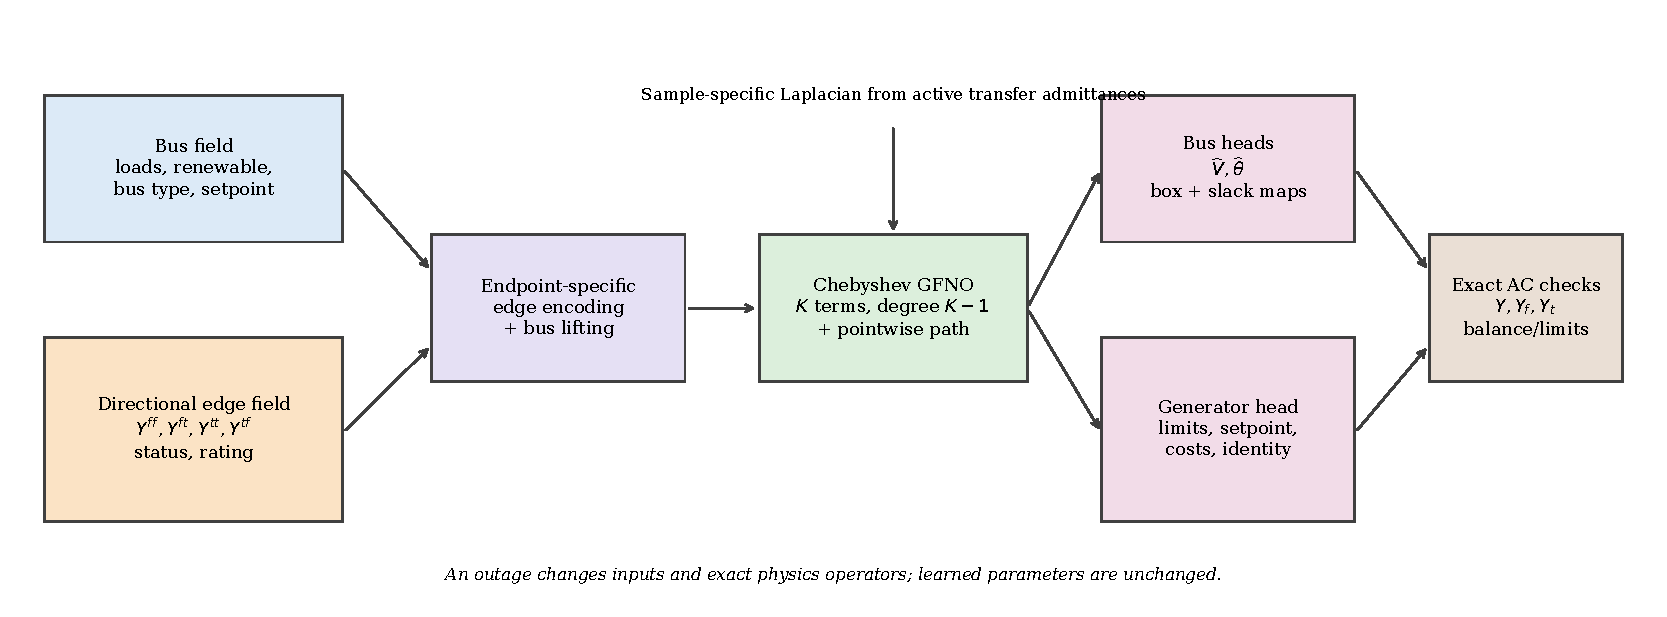
\includegraphics[width=0.95\textwidth]{figures/fig_architecture.pdf}
  \caption{Topology-conditioned GFNO-PINO architecture. A line outage changes
  the edge status, the graph Laplacian, and the exact admittance operators
  supplied to the loss; learned parameters are unchanged.}
  \label{fig:arch}
\end{figure*}

\subsection{Physics-informed loss function}
\label{subsec:loss}

All powers in the network equations are in per unit on the case base
$S_{\mathrm{base}}$; generator powers are converted to MW before evaluating
the supplied cost polynomial. To prevent a soft-constrained model from being
rewarded for reducing cost by shedding power, the implemented economic term is
one-sided samplewise normalized regret,
\begin{equation}
  \mathcal{L}_{\mathrm{economic}}
  =
  \mean_b
  \left[
  \relu\left(
  \frac{C(\widehat P_b^g)-C(P_b^{g,\mathrm{ref}})}
       {\max(|C(P_b^{g,\mathrm{ref}})|,C_{\mathrm{scale}})}
  \right)
  \right]^2,
  \label{eq:loss_cost}
\end{equation}
where $P_b^{g,\mathrm{ref}}$ is the locally converged IPOPT dispatch and
$C_{\mathrm{scale}}=1$ currency unit per hour. The ReLU is evaluated before
the batch mean, so an over-cost sample cannot be cancelled by an under-cost
sample; the formula also remains correct when a reference cost is negative.
Lower predicted cost is not rewarded unless the other objectives retain the
solver-informed dispatch and satisfy the AC equations.
Let $r_{i,b}^P$ and $r_{i,b}^Q$ be the left side minus the right side of
Eqs.~\eqref{eq:p_balance} and \eqref{eq:q_balance}. The equality residual is
\begin{equation}
  \mathcal{L}_{\mathrm{powerflow}}
  =
  \mean_{(b,i)\,\mathrm{valid}}
  \left[
    (r_{i,b}^P)^2+(r_{i,b}^Q)^2
  \right].
  \label{eq:loss_pf}
\end{equation}
The two-ended thermal excess and penalty are
\begin{align}
  \nu_{a,b}^{S}
  &=
  \relu\left(
    \max\{|\widehat S_{a,b}^f|,
           |\widehat S_{a,b}^t|\}
    -S_{a}^{\max}
  \right),
  \nonumber\\
  \mathcal{L}_{\mathrm{thermal}}
  &=
  \mean_{(b,a)\in\mathcal{B}_{S}}
  (\nu_{a,b}^{S})^2,
  \label{eq:loss_thermal}
\end{align}
where $\mathcal{B}_{S}$ contains only active, rated branches. The
angle-difference excess is trained for every active branch:
\begin{align}
  \nu_{a,b}^{\theta}
  ={}&
  \relu\left(
    \underline{\Delta\theta}_a
    -(\widehat\theta_{f(a),b}-\widehat\theta_{t(a),b})
  \right)
  \nonumber\\
  &+
  \relu\left(
    (\widehat\theta_{f(a),b}-\widehat\theta_{t(a),b})
    -\overline{\Delta\theta}_a
  \right),
  \nonumber\\
  \mathcal{L}_{\mathrm{angle}}
  ={}&
  \mean_{(b,a):s_a(z_b)=1}
  (\nu_{a,b}^{\theta})^2.
  \label{eq:loss_angle}
\end{align}
Although voltage boxes are
enforced by the output layer, their reported diagnostic is
\begin{align}
  \nu_{i,b}^{V}
  &=
  \relu(V_i^{\min}-\widehat V_{i,b})
  +\relu(\widehat V_{i,b}-V_i^{\max}),
  \nonumber\\
  \mathcal{L}_{\mathrm{voltage}}
  &=
  \mean_{b,i}(\nu_{i,b}^{V})^2.
  \label{eq:loss_voltage}
\end{align}
An analogous generator-box diagnostic is also logged. Neither identically zero
hard-box diagnostic participates in adaptive loss balancing. Given solver
labels $u_b^{\mathrm{ref}}$, the warm-start term is
\begin{equation}
  \mathcal{L}_{\mathrm{data}}
  =
  \frac{1}{4}\sum_{q\in\{V,\theta,P^g,Q^g\}}
  \mean_{(b,k)\,\mathrm{valid}}
  (\widehat q_{b,k}-q_{b,k}^{\mathrm{ref}})^2.
  \label{eq:loss_data}
\end{equation}
The total training objective is
\begin{equation}
  \begin{aligned}
    \mathcal{L}_{\mathrm{total}}
    ={}&
    \lambda_{\mathrm{cost}}\mathcal{L}_{\mathrm{economic}}
    +\lambda_{\mathrm{pf}}s_{\mathrm{pf}}\mathcal{L}_{\mathrm{powerflow}}
    +\lambda_{\mathrm{thermal}}s_{\mathrm{th}}\mathcal{L}_{\mathrm{thermal}}\\
    &+\lambda_{\mathrm{angle}}\mathcal{L}_{\mathrm{angle}}
    +\lambda_{\mathrm{data}}\mathcal{L}_{\mathrm{data}}.
  \end{aligned}
  \label{eq:total_loss}
\end{equation}

During physics epoch $e\in\{1,\ldots,E_p\}$, define the exact objectives
supplied to both the GradNorm update and the subsequent model update as
\begin{equation}
  \begin{aligned}
  (\widetilde{\mathcal L}_m)_m
  =\big(&
    \mathcal L_{\mathrm{economic}},
    s_{\mathrm{pf}}(e)\mathcal L_{\mathrm{powerflow}},
    s_{\mathrm{th}}(e)\mathcal L_{\mathrm{thermal}},\\[-2pt]
    &\mathcal L_{\mathrm{angle}},
    \mathcal L_{\mathrm{data}}
  \big),
  \end{aligned}
  \label{eq:annealed_objectives}
\end{equation}
where $s_{\mathrm{pf}}(e)=1+9e/E_p$ and
$s_{\mathrm{th}}(e)=1+4e/E_p$. Thus annealing changes the model gradient as
well as the weight-balancing dynamics. To make GradNorm
\cite{chen2018gradnorm} well-defined when a constraint loss is initially zero,
objective $m$ enters the active set $\mathcal A$ only on the first step
$t_m$ for which its detached value exceeds $\varepsilon=10^{-8}$; its baseline
is then $\widetilde{\mathcal L}_{m,0}
=\widetilde{\mathcal L}_m(t_m)$. Let
$g_m=\|\nabla_{\Theta_s}
  (\lambda_m\widetilde{\mathcal L}_m)\|_2$. Here
$\Theta_s=W_{\mathrm{lift}}$ is exactly the \texttt{lift.weight} matrix for
GFNO and spatial-GNN models; the fixed-topology PINN uses
\texttt{network.0.weight}. For the current active set, the positive weights
are normalized as $\sum_{m\in\mathcal A}\lambda_m=|\mathcal A|$; inactive
weights are exactly zero and do not enter this normalization. Let
\begin{equation}
 \rho_m=
 \frac{
  (\operatorname{stopgrad}\widetilde{\mathcal L}_m+\varepsilon)/
  (\widetilde{\mathcal L}_{m,0}+\varepsilon)}
 {\mean_{j\in\mathcal A}
  [(\operatorname{stopgrad}\widetilde{\mathcal L}_j+\varepsilon)/
  (\widetilde{\mathcal L}_{j,0}+\varepsilon)]}.
 \label{eq:relative_training_rate}
\end{equation}
The weight update minimizes
\begin{equation}
  \mathcal{L}_{\mathrm{GN}}
  =
  \sum_{m\in\mathcal A}
  \left|
    g_m-\overline g\,\rho_m^\alpha
  \right|,
  \qquad
  \overline g=\mean_{m\in\mathcal A} g_m,
  \label{eq:gradnorm}
\end{equation}
with $\alpha=0.5$ and a stop-gradient target
$\overline g\rho_m^\alpha$. If fewer than two objectives are active, the weight
update is zero. The subsequent model update detaches the normalized weights;
therefore the model and weight optimizers cannot differentiate through each
other. Every raw loss, annealing factor, and effective weight is retained in
the run artifacts; active-set transitions are deterministic from the archived
losses and $\varepsilon$.

\subsection{Hard-constraint enforcement layer}
\label{subsec:hard}

For unconstrained decoder values
$a_i^V,a_g^P,a_g^Q\in\R$, the independent box constraints are enforced by
\begin{align}
  \widehat V_i
  &=
  V_i^{\min}
  +(V_i^{\max}-V_i^{\min})\sigma(a_i^V),
  \label{eq:hard_v}\\
  \widehat P_g^g
  &=
  P_g^{\min}
  +(P_g^{\max}-P_g^{\min})\sigma(a_g^P),
  \label{eq:hard_p}\\
  \widehat Q_g^g
  &=
  Q_g^{\min}
  +(Q_g^{\max}-Q_g^{\min})\sigma(a_g^Q),
  \label{eq:hard_q}
\end{align}
where $\sigma$ is the logistic sigmoid. For finite logits this map reaches the
open interval, not its endpoints. It guarantees membership in the closed box
but cannot represent a reference solution exactly at an active bound; this
active-set limitation is quantified in Section~\ref{sec:results}. If
$\widetilde\theta$ is the raw angle vector, the reference is imposed by
\begin{equation}
  \widehat\theta_i
  =
  \widetilde\theta_i
  -\widetilde\theta_{i_{\mathrm{ref}}}.
  \label{eq:hard_slack}
\end{equation}
Equations~\eqref{eq:hard_v}--\eqref{eq:hard_slack} guarantee the voltage and
generator boxes and slack reference up to floating-point precision. They do
\emph{not} guarantee Eqs.~\eqref{eq:p_balance},
\eqref{eq:q_balance}, \eqref{eq:thermal_limits}, or
\eqref{eq:angle_limits}; those coupled non-convex constraints remain
approximate and must be measured after inference.

\subsection{Training procedure}

Training uses two phases. The first phase supplies a stable solver-informed
initialization. The second phase jointly optimizes economic quality and
physical consistency, with adaptive weights reducing sensitivity to disparate
units and gradient scales. Topology IDs are sampled only from the training
partition.

\begin{algorithm}[t]
  \caption{Supervised warm start and physics-informed fine-tuning}
  \label{alg:training}
  \begin{algorithmic}[1]
    \REQUIRE Topology-disjoint datasets
      $\mathcal{D}_{\mathrm{tr}},\mathcal{D}_{\mathrm{val}}$;
      model $\mathcal{G}_\Theta$; warm epochs $E_w$; physics epochs $E_p$
    \STATE Initialize $\Theta$, optimizer, scheduler, and adaptive
      log-weights $\{\log\lambda_m\}$
    \FOR{$e=1$ to $E_w$}
      \FOR{mini-batch $\mathcal{Q}\subset\mathcal{D}_{\mathrm{tr}}$}
        \STATE Predict $\widehat u_b=\mathcal{G}_\Theta(X_b,E_b,z_b,\mathcal{M}_{\mathrm{pred},b})$
        \STATE Update $\Theta$ using $\mathcal{L}_{\mathrm{data}}$
      \ENDFOR
      \STATE Evaluate label error and AC residuals on $\mathcal{D}_{\mathrm{val}}$
    \ENDFOR
    \FOR{$e=1$ to $E_p$}
      \FOR{mini-batch $\mathcal{Q}\subset\mathcal{D}_{\mathrm{tr}}$}
        \STATE Predict $\widehat u_b$ with sample-specific topology
        \STATE Compute Eqs.~\eqref{eq:loss_cost}--\eqref{eq:loss_data}
          using $Y_b,Y_{f,b},Y_{t,b}$
        \STATE Apply $s_{\mathrm{pf}}(e)$ and $s_{\mathrm{th}}(e)$; activate
          nonzero objectives and record their first positive baselines
        \STATE Update $\{\log\lambda_m\}$ using Eq.~\eqref{eq:gradnorm}
          with detached targets
        \STATE Update $\Theta$ using Eq.~\eqref{eq:total_loss};
          detach $\lambda_m$ and clip the global gradient norm
      \ENDFOR
      \STATE Save the checkpoint minimizing
        $5\mathcal L_{\mathrm{data}}+\mathcal L_{\mathrm{powerflow}}
        +\mathcal L_{\mathrm{thermal}}+\mathcal L_{\mathrm{angle}}$
    \ENDFOR
    \RETURN Best validation checkpoint and all component-wise logs
  \end{algorithmic}
\end{algorithm}

\section{Case study and experimental setup}
\label{sec:experiments}

\subsection{Test systems}

Experiments are configured for the IEEE 30-, 57-, 118-, and 300-bus systems
distributed through pandapower and compatible MATPOWER data
\cite{zimmerman2011matpower,thurner2018pandapower}. Table~\ref{tab:systems}
reports structural facts extracted by the released data pipeline. ``Eligible
N-1'' counts non-islanding outages of elements represented as lines in each
pandapower case; transformer outages are not included in the present
contingency set.

\begin{table*}[t]
  \centering
  \caption{Test-system characteristics used by the data generator.}
  \label{tab:systems}
  \begin{tabular}{lrrrrrr}
    \toprule
    Case & Buses & Gen. & Loads & Lines & Trafos & Eligible N-1 \\
    \midrule
    IEEE 30  & 30  & 6  & 20  & 41  & 0   & 38  \\
    IEEE 57  & 57  & 7  & 42  & 63  & 17  & 62  \\
    IEEE 118 & 118 & 54 & 99  & 173 & 13  & 166 \\
    IEEE 300 & 300 & 69 & 193 & 283 & 128 & 253 \\
    \bottomrule
  \end{tabular}
\end{table*}

\begin{table*}[t]
  \centering
  \caption{Executed pilot training configurations. Width is the latent channel
  count; $K$ is the number of Chebyshev terms and the polynomial degree is
  $K-1$.}
  \label{tab:hyperparameters}
  \begin{tabular}{lrrrrr}
    \toprule
    Case & Width & Depth & $K$ & Batch & Warm/physics epochs \\
    \midrule
    IEEE 30  & 64 & 4 & 3 & 16 & 12/18 \\
    IEEE 57  & 64 & 4 & 3 & 12 & 12/18 \\
    IEEE 118 & 96 & 4 & 3 & 8  & 12/18 \\
    IEEE 300 & 96 & 4 & 3 & 4  & 12/18 \\
    \bottomrule
  \end{tabular}
\end{table*}

Every neural experiment uses seeds 2026--2030, Python 3.12.13,
single-precision PyTorch 2.13.0 with Compute Unified Device Architecture
(CUDA) 12.6, and an NVIDIA GeForce RTX 3050 6 GB Laptop graphics processing
unit (GPU). Data handling uses pandapower 3.5.4, NumPy 2.4.6, SciPy
1.18.0, and pandas 2.3.3. Hyperparameters were fixed before the repeated runs.
The checkpoint, configuration, parameter count, training history, software
version, device, and runtime are archived for each case--model--seed
combination. AdamW uses learning rates
$10^{-3},10^{-3},8{\times}10^{-4},6{\times}10^{-4}$ from 30 to 300 buses,
weight decay $10^{-5}$, and global gradient-norm clipping at 1.0. A
30-epoch cosine schedule has no restart or early stopping. The adaptive-weight
optimizer is Adam with learning rate 0.01. Dropout is 0.05; the directional
edge conditioner comprises separate from/to two-layer MLPs of
$10\!\rightarrow\!d\!\rightarrow\!d$ channels with GELU.

\begin{table*}[t]
  \centering
  \caption{Model-specific fitting and checkpoint-selection protocol. Parameter
  counts are ordered as IEEE 30/57/118/300. ``Best'' means the minimum score
  over all 30 completed epochs; no early-stopping rule was used.}
  \label{tab:model_protocol}
  \scriptsize
  \resizebox{\textwidth}{!}{%
  \begin{tabular}{lccccc}
    \toprule
    Model & Fitting rows/topologies & Validation rows/topologies &
    Training objective & Checkpoint score & Parameters \\
    \midrule
    Base-only PINN & 10/base only & 2/base only &
      12 supervised + 18 physics &
      $5L_{\rm data}+L_{\rm pf}+L_{\rm th}+L_{\rm angle}$ &
      28\,424/45\,888/142\,712/320\,706 \\
    Topology-blind GFNO & 84 or 96/8 IDs & 12/1 held-out ID &
      12 supervised + 18 physics & same &
      90\,116/90\,116/199\,684/199\,684 \\
    Plain GNN & 84 or 96/8 IDs & 12/1 held-out ID &
      12 supervised + 18 physics & same &
      57\,348/57\,348/125\,956/125\,956 \\
    Data-only GFNO & 84 or 96/8 IDs & 12/1 held-out ID &
      30 supervised & same physics-aware score &
      90\,116/90\,116/199\,684/199\,684 \\
    GFNO-PINO & 84 or 96/8 IDs & 12/1 held-out ID &
      12 supervised + 18 physics & same &
      90\,116/90\,116/199\,684/199\,684 \\
    \bottomrule
  \end{tabular}}
\end{table*}

\subsection{Contingency and scenario generation}
\label{subsec:scenario_generation}

For every in-service line, the generator creates a copied network, sets that
line out of service, and tests graph connectivity while retaining transformers
and parallel circuits. Islanding outages are recorded and excluded. To maintain
a fixed edge axis, topology artifacts preserve the full base-case
$\Bset=\Lset\cup\Xset$ canonical branch list, set the selected physical-line
status to zero, and retain status one for fixed transformers. Component type and
the physical-line-to-branch index map are stored explicitly. Exact $Y$, $Y_f$, and $Y_t$
operators are stored once per topology; scenario files reference them by
topology ID.

The pilot cap is deterministic and was applied \emph{before} the split: the
base topology and the first 11 non-islanding outages encountered in
pandapower line-index order were retained. No random or severity-based outage
selection was used. NumPy's \texttt{default\_rng(2026)} then shuffled those 11
outage IDs and the nominal 0.70/0.15/0.15 fractions were floored, yielding
7/1/3 outage IDs plus the base topology in training. This convenience sample
does not represent the full eligible N-1 distribution; Table~\ref{tab:systems}
reports the much larger eligible counts.

Loads are perturbed by bounded, spatially correlated multipliers. A
squared-exponential kernel is formed from all-pairs graph distances and
projected onto a positive-semidefinite eigenspectrum before sampling. Configured
ranges are $\pm30\%$, $\pm35\%$, $\pm40\%$, and $\pm20\%$ for the four pilot
systems, respectively. The IEEE 300-bus range was reduced from the initially
configured $\pm50\%$ after repeated IPOPT iteration-limit failures and is
therefore a less stressed pilot, not a like-for-like stress test. Active and
reactive demand at a load are scaled together to retain its base power factor.
Renewable injections are allocated at generator or load buses and treated as
fixed, unity-power-factor injections. All reported experiments use the
generator's correlated synthetic-diurnal profile, with capacity fractions
0.20, 0.20, 0.25, and 0.15, respectively. No claim of validation on real NREL
or operational renewable data is made. Specifically, at hour $h$, the common
clear-sky factor is
$\max\{0,\sin[\pi(h-6)/12]\}$, multiplied by an independently sampled
$\operatorname{Beta}(5,2)$ cloud factor and site factors
$\mathcal{N}(1,0.08^2)$, then clipped to $[0,1]$. The graph-kernel correlation
lengths for load sampling are 3.0, 3.5, 4.0, and 5.0 hops.

Each feasible scenario is solved with PowerModels' polar AC formulation and
IPOPT \cite{coffrin2018powermodels,wachter2006ipopt}. Solver termination status,
objective, tolerances, and wall-clock time are retained. The pandapower/PYPOWER
backend is available for pipeline debugging but must not be merged into a table
labelled ``IPOPT.'' DC-OPF is solved separately for its speed and approximation
baseline using pandapower 3.5.4 \texttt{rundcopp} with its default PYPOWER
backend and power tolerance $10^{-10}$. It minimizes the imported active-power
generation cost subject to the linearized active-power/angle model and active
branch loading constraints; voltage magnitude and reactive-power variables
are absent. No custom angle reference, initialization, or solver option was
passed beyond pandapower defaults. Its recorded value is therefore a DC
approximation and timing baseline, never an AC-feasibility claim.

Topology IDs, not individual rows, are split once and then held fixed across
models and seeds. The realized split is 8/1/3 topology IDs
(66.7\%/8.3\%/25.0\%) for each case, with the base topology in training.
IEEE 30 has 7/1/3 \emph{usable} topology IDs because one assigned training
outage has no converged sample. The corresponding sample counts are
84/12/36 for IEEE 30 and 96/12/36 for the other cases. Thus, every reported
test contingency is absent from training. The exact topology names, outage
indices, split assignments, connectivity decisions, and sample counts are
published in each case's \texttt{topology\_manifest.csv}; the percentages are
descriptive, not an unrealized nominal target.

\subsection{Baselines}

The comparison includes:
\begin{enumerate}
  \item \textbf{IPOPT AC-OPF}: locally converged dispatch, objective,
    constraint, and wall-clock reference; no global-optimality certificate is
    claimed.
  \item \textbf{DC-OPF}: linear speed baseline; reactive and voltage feasibility
    are not attributed to this model.
  \item \textbf{Fixed-topology PINN}: a dense PINN trained only on base-topology
    scenarios and evaluated without retraining on held-out outages.
  \item \textbf{Topology-blind GFNO}: a parameter-matched GFNO trained on the
    same multi-topology rows as GFNO-PINO but supplied one fixed base-topology
    edge field and Laplacian for every sample.
  \item \textbf{Plain GNN}: the same topology inputs and hard output head, with
    spatial mean aggregation replacing Chebyshev spectral filters.
  \item \textbf{Data-only GFNO}: the evaluated graph-spectral architecture trained
    throughout on solver-label mean-square error, without physics fine-tuning.
\end{enumerate}
The matched topology-blind GFNO is the causal test of topology input. The
base-only PINN is retained only as a practically relevant out-of-distribution
reference: because it sees 12 base rows rather than the multi-topology training
set, its comparison is intentionally not attributed solely to architecture.
The plain GNN isolates spectral versus spatial propagation, and the data-only
GFNO isolates physics fine-tuning. Width and depth are shared where the
architecture permits; parameter counts are archived for every checkpoint.

\subsection{Evaluation metrics}

For sample $b$, the signed reference-cost difference is
\begin{equation}
  \begin{aligned}
    \Delta C_b^{\mathrm{ref}}(\%)
    &=
    100
    \frac{C(\widehat P_b^g)-C(P_b^{g,\mathrm{ref}})}
    {\max(|C(P_b^{g,\mathrm{ref}})|,C_{\mathrm{scale}})},\\
    C_{\mathrm{scale}}&=1\ {\rm currency/hour}.
  \end{aligned}
  \label{eq:reference_cost_difference}
\end{equation}
A negative value does not establish superiority if the prediction is
infeasible. The per-bus complex-power-balance mismatch is
\begin{equation}
  d_{i,b}=\sqrt{(r^P_{i,b})^2+(r^Q_{i,b})^2},
  \qquad
  d_b^{\max}=\max_{i\in\Nset}d_{i,b}.
  \label{eq:balance_metric}
\end{equation}
Within seed $r$, ``mean bus'' is
$\overline d_{\mathrm{bus},r}=(B_r|\Nset|)^{-1}
\sum_{b=1}^{B_r}\sum_{i\in\Nset}d_{i,b}$ and ``mean max.'' is
$B_r^{-1}\sum_b d_b^{\max}$. P95 and worst are computed over the $B_r=36$
held-out samples within each seed. Tables then report the arithmetic mean of
each within-seed statistic across five seeds; a displayed $\pm$ value is the
sample standard deviation across those five seed statistics. Separate
active/reactive maxima use the same nesting. This is a power-balance mismatch
in p.u.; it is not labeled a current residual. A
telescoping angle-cycle identity is not reported as a performance metric.
All reported standard deviations and seed-resampling intervals are computed
from only five training seeds per case. They are descriptive summaries of
algorithmic variation within this fixed pilot dataset and training budget, not
frequentist population-confidence statements.

For constraint class $c$, the violation rate and magnitude are
\begin{align}
  R_c
  &=
  \frac{\#\{k:v_{c,k}>\tau_c\}}{\#\{k\}},
  \label{eq:violation_rate}\\
  M_c^{\max}
  &=
  \max_k v_{c,k},
  \qquad
  M_c^{\mathrm{mean}}
  =
  \mean_k v_{c,k},
  \label{eq:violation_magnitude}
\end{align}
for voltage, thermal, generator, and branch angle-difference constraints. The
class threshold is $\tau_c=10^{-6}$ for every inequality (radians for angle,
p.u. otherwise). Within a seed, $k$ ranges over all valid sample--element pairs
for rates, while the reported magnitude is the within-seed maximum followed by
the five-seed mean. The AC-feasibility proxy requires
$d_b^{\max}\leq\tau_{\mathrm{bal}}=10^{-3}$ p.u. and every represented
inequality excess to be at most $\tau_c$.
Latency is measured after ten warm-up passes with batch size one and CUDA
device synchronization, then summarized across the 36 test samples and five
seeds. Neural timing excludes topology construction, host--device transfer,
constraint verification, and feasibility restoration; stored solver timing is
CPU wall time. Results are grouped by bus count and topology ID. Accuracy on
the test partition is the primary unseen-topology result; random row-wise
splits are not reported as contingency generalization.

\section{Results and discussion}
\label{sec:results}

\subsection{Executed benchmark and numerical verification}

The executed pipeline produced 564 converged AC-OPF labels and 3600 neural
test evaluations (4 systems $\times$ 5 models $\times$ 5 seeds $\times$ 36
held-out samples). All AC references were solved with PowerModels 0.21.6,
JuMP 1.31.1, and IPOPT 1.15.0 using the polar formulation, optimality and
constraint-violation tolerances of $10^{-8}$, and the MUMPS linear solver. The
released verification suite passes 25 tests. These include an analytic two-bus
balance, independent explicit $G$--$B$ injection equations, directional
two-ended branch flows with phase shift, automatic differentiation, hard-box
enforcement, angle-limit excess, zero-safe adaptive weighting,
topology-disjoint splitting, outage masking, the MATPOWER writer, and numerical
agreement with a converged IEEE 30-bus power flow.

\begin{table*}[t]
  \centering
  \caption{Executed topology-disjoint pilot dataset. ``Failed'' counts solver
  attempts rejected before the target number of converged labels was reached.}
  \label{tab:pilot_data}
  \begin{tabular}{lrrrrrrrr}
    \toprule
    Case & Target & Converged & Failed & Usable topol. &
    Train & Validation & Test & Test topol. \\
    \midrule
    IEEE 30  & 144 & 132 & 154 & 11 & 84 & 12 & 36 & 3 \\
    IEEE 57  & 144 & 144 & 46  & 12 & 96 & 12 & 36 & 3 \\
    IEEE 118 & 144 & 144 & 0   & 12 & 96 & 12 & 36 & 3 \\
    IEEE 300 & 144 & 144 & 0   & 12 & 96 & 12 & 36 & 3 \\
    \bottomrule
  \end{tabular}
\end{table*}

Table~\ref{tab:pilot_data} exposes two important selection effects. First, the
IEEE 30 outage \texttt{line\_9\_out} produced no converged sample in 60
attempts and was retained only as a zero-count training topology; it did not
enter the test set. Second, the imported IEEE 57 and IEEE 300 cases required
explicit voltage ranges of $[0.8,1.1]$ and $[0.9,1.1]$ p.u., respectively, to
obtain a runnable pilot. Together with the reduced IEEE 300 load range, these
adjustments mean that cross-system comparisons measure computational scaling,
not identical electrical stress. Every test set nevertheless contains three
contingencies absent from its corresponding training set.
The source constraint inventories show MATPOWER angle bounds of
$[-360^\circ,360^\circ]$ on every represented branch, so they are
nonrestrictive in these four cases. Angle excess is still evaluated and
included in the proxy so that restrictive source cases cannot be silently
omitted.

\subsection{Economic performance}

\begin{table*}[t]
\centering
\caption{Signed reference-cost difference (\%) on topology-disjoint test sets. Neural entries are mean $\pm$ standard deviation across five training seeds; negative values from infeasible predictions are not optimality gains.}
\label{tab:optimality}
\scriptsize
\begin{tabular}{lrrrr}
\toprule
Method & IEEE 30 & IEEE 57 & IEEE 118 & IEEE 300 \\
\midrule
DC-OPF & -2.65 & -3.16 & -2.94 & -2.03 \\
Base-only PINN (OOD) & 1.97 $\pm$ 2.66 & -7.04 $\pm$ 3.74 & 28.50 $\pm$ 1.68 & 0.45 $\pm$ 0.48 \\
Topology-blind GFNO & -34.63 $\pm$ 5.03 & -22.53 $\pm$ 2.74 & -24.43 $\pm$ 6.28 & -22.71 $\pm$ 6.32 \\
Plain GNN & -26.78 $\pm$ 6.25 & -19.08 $\pm$ 3.90 & -21.02 $\pm$ 11.23 & -14.33 $\pm$ 7.53 \\
Data-only GFNO & 3.15 $\pm$ 0.37 & -3.73 $\pm$ 0.90 & 4.88 $\pm$ 0.96 & 0.67 $\pm$ 1.26 \\
GFNO-PINO & -35.17 $\pm$ 4.15 & -25.32 $\pm$ 1.72 & -26.56 $\pm$ 10.22 & -20.92 $\pm$ 6.63 \\
\bottomrule
\end{tabular}
\end{table*}


Across DC-OPF and the five neural models,
Table~\ref{tab:optimality} compares the signed reference-cost difference of
Eq.~\eqref{eq:reference_cost_difference}; neural entries are five-seed means
and standard deviations. A negative value from a neural surrogate
is interpreted only jointly with Tables~\ref{tab:violations}
and~\ref{tab:balance}: an infeasible dispatch can appear cheaper by failing to
supply losses or demand. The same
caution applies to DC-OPF because it omits reactive power, voltage magnitudes,
and AC losses. A feasibility-conditioned reference-cost difference is reported only when at
least one prediction satisfies the declared proxy; otherwise it is undefined,
not zero. Consequently, cost statistics alone do not establish economic
superiority over IPOPT. GFNO-PINO's signed reference-cost differences are
$-35.17\pm4.15\%$, $-25.32\pm1.72\%$, $-26.56\pm10.22\%$, and
$-20.92\pm6.63\%$ from 30 to 300 buses; the corresponding mean absolute
differences are 35.17\%, 26.44\%, 27.85\%, and 21.13\%. Since no GFNO-PINO sample is
proxy-feasible, every feasibility-conditioned difference is undefined.

\subsection{Physical residuals and constraint violations}

\begin{table*}[t]
\centering
\caption{GFNO-PINO inequality diagnostics on unseen topologies. Each entry is violation rate (\%)/mean seed-maximum excess (p.u., except angle in rad). The AC-feasible column additionally requires a $10^{-3}$ p.u. maximum complex-power-balance mismatch.}
\label{tab:violations}
\scriptsize
\begin{tabular}{lrrrrr}
\toprule
System & Voltage & Thermal & Generator & Angle & AC feasible (\%) \\
\midrule
IEEE 30 & 0.00/0.00e+00 & 1.00/8.59e-03 & 0.00/0.00e+00 & 0.00/0.00e+00 & 0.0 \\
IEEE 57 & 0.00/0.00e+00 & 0.00/0.00e+00 & 0.00/0.00e+00 & 0.00/0.00e+00 & 0.0 \\
IEEE 118 & 0.00/0.00e+00 & 0.00/0.00e+00 & 0.00/0.00e+00 & 0.00/0.00e+00 & 0.0 \\
IEEE 300 & 0.00/0.00e+00 & 0.00/0.00e+00 & 0.00/0.00e+00 & 0.00/0.00e+00 & 0.0 \\
\bottomrule
\end{tabular}
\end{table*}

\begin{table*}[t]
\centering
\caption{GFNO-PINO complex-power-balance diagnostics in p.u. on unseen topologies. Mean max. is mean $\pm$ seed standard deviation; P95 and worst are five-seed means of within-seed held-out statistics.}
\label{tab:balance}
\scriptsize
\begin{tabular}{lrrrrrr}
\toprule
System & Mean bus & Mean max. & P95 max. & Worst max. & Mean max. $|r^P|$ & Mean max. $|r^Q|$ \\
\midrule
IEEE 30 & 0.085 & 0.281 $\pm$ 0.011 & 0.324 & 0.334 & 0.178 & 0.232 \\
IEEE 57 & 0.255 & 1.684 $\pm$ 0.107 & 2.415 & 2.619 & 1.644 & 0.843 \\
IEEE 118 & 0.266 & 0.890 $\pm$ 0.112 & 1.020 & 1.121 & 0.814 & 0.668 \\
IEEE 300 & 0.905 & 5.959 $\pm$ 3.360 & 6.221 & 6.351 & 5.046 & 4.696 \\
\bottomrule
\end{tabular}
\end{table*}

\begin{table*}[t]
\centering
\caption{Observed effect of physics fine-tuning on mean sample-maximum complex-power-balance mismatch (p.u.). Model columns are mean $\pm$ seed standard deviation. Paired reduction compares identical seeds. All five seed effects are shown; the final column is a deterministic 10,000-resample percentile interval used descriptively, not as population-level confidence.}
\label{tab:physics_effect}
\scriptsize
\resizebox{\textwidth}{!}{%
\begin{tabular}{lrrrrr}
\toprule
System & Data-only GFNO & GFNO-PINO & Paired mean (\%) & Seed effects 2026--2030 (\%) & Seed-resampling interval (\%) \\
\midrule
IEEE 30 & 1.107 $\pm$ 0.177 & 0.281 $\pm$ 0.011 & 74.1 $\pm$ 4.6 & 77.3,72.1,67.0,77.0,77.2 & [70.0, 77.2] \\
IEEE 57 & 4.606 $\pm$ 0.212 & 1.684 $\pm$ 0.107 & 63.4 $\pm$ 2.3 & 65.8,65.1,60.2,63.9,62.0 & [61.5, 65.1] \\
IEEE 118 & 6.092 $\pm$ 0.284 & 0.890 $\pm$ 0.112 & 85.4 $\pm$ 2.0 & 82.8,84.4,85.0,88.1,86.5 & [83.9, 87.0] \\
IEEE 300 & 55.999 $\pm$ 9.736 & 5.959 $\pm$ 3.360 & 89.3 $\pm$ 6.1 & 93.5,86.4,92.9,93.9,79.9 & [83.9, 93.5] \\
\bottomrule
\end{tabular}
}
\end{table*}

\begin{table*}[t]
\centering
\caption{GFNO-PINO error stratified by active reference boxes on the unseen-topology
test sets. A reference is ``near bound'' when it lies within $10^{-4}$ p.u. of
either limit. Fractions use the 36 distinct references per case; active/inactive
MAEs pool the five paired model seeds (p.u.).}
\label{tab:active_bounds}
\scriptsize
\begin{tabular}{lrrrrrr}
\toprule
System & \multicolumn{3}{c}{Reference near bound (\%): $V/P^g/Q^g$} &
\multicolumn{3}{c}{MAE active/inactive: $V/P^g/Q^g$} \\
\cmidrule(lr){2-4}\cmidrule(lr){5-7}
 & $V$ & $P^g$ & $Q^g$ & $V$ & $P^g$ & $Q^g$ \\
\midrule
IEEE 30  & 4.81 & 0.46 & 6.02 & 0.022/0.031 & 0.346/0.092 & 0.263/0.086 \\
IEEE 57  & 4.53 & 21.43 & 47.62 & 0.071/0.070 & 0.620/0.466 & 0.211/0.394 \\
IEEE 118 & 7.11 & 38.68 & 21.86 & 0.048/0.042 & 0.180/0.525 & 0.198/0.204 \\
IEEE 300 & 9.80 & 9.46 & 40.66 & 0.098/0.066 & 0.393/0.682 & 0.285/0.476 \\
\bottomrule
\end{tabular}
\end{table*}


The hard output transformations make voltage and generator box excess zero up
to floating-point precision; this is a parameterization check, not learned AC
feasibility. Table~\ref{tab:violations} separately reports thermal and
angle-difference excess and the Euclidean active/reactive balance mismatch of
Eq.~\eqref{eq:balance_metric}. The latter must not be confused with current
magnitude or with either component alone. Any nonzero mismatch beyond the
declared threshold shows why bounded heads and a small supervised error cannot
substitute for a coupled AC-feasibility layer.

Table~\ref{tab:active_bounds} addresses the logistic-head endpoint limitation.
Active reference boxes are common for reactive dispatch in IEEE 57 and 300 and
for active dispatch in IEEE 118. The stratified errors do not show one
universal direction, but several active groups are materially harder (notably
$P^g$ and $Q^g$ in IEEE 30 and $P^g$ in IEEE 57). A projection or hard-sigmoid
head could represent endpoints, but would still not guarantee the coupled AC
equalities; changing the head would require retraining and is not retrospectively
applied to these archived runs.

GFNO-PINO's mean sample-maximum balance mismatches are
$0.281\pm0.011$, $1.684\pm0.107$, $0.890\pm0.112$, and
$5.959\pm3.360$ p.u.; five-seed mean within-seed worst values are 0.334,
2.619, 1.121, and 6.351 p.u.

For identical seeds, the paired reductions relative to the data-only GFNO are
$74.1\pm4.6\%$, $63.4\pm2.3\%$, $85.4\pm2.0\%$, and
$89.3\pm6.1\%$. Table~\ref{tab:physics_effect} shows every paired seed effect
and the deterministic seed-resampling intervals [70.0, 77.2]\%,
[61.5, 65.1]\%, [83.9, 87.0]\%, and [83.9, 93.5]\%. All 20 observed paired
effects are positive, but five seeds are too few to support population-level
coverage or robustness claims. The remaining mismatch is two to four orders of magnitude
above the $10^{-3}$ p.u. threshold. GFNO-PINO has a 1.0\% thermal-violation
rate on IEEE 30 with a five-seed mean maximum excess of 0.00859 p.u. Given the
small held-out sample count (36 per seed), this rate should be treated as
indicative rather than a precise estimate; per-seed violation counts are
archived in the topology-resolved CSVs for independent inspection. The other
three systems have no measured thermal excess. Voltage, generator, and the
nonrestrictive source angle boxes have zero excess. The resulting feasibility
  rate is 0\% for every learned model and case.

\begin{figure}[t]
  \centering
  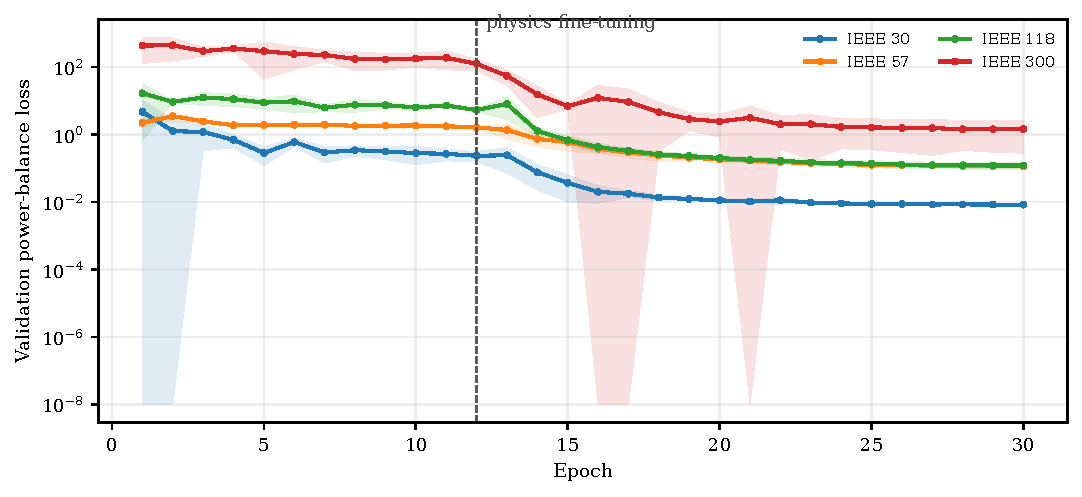
\includegraphics[width=\columnwidth]
    {figures/fig_residual_convergence.pdf}
  \caption{Five-seed mean validation power-balance loss during the 12-epoch
  supervised warm start and 18-epoch physics fine-tuning. Shading is one
  standard deviation across training seeds.}
  \label{fig:residual_convergence}
\end{figure}

\begin{figure}[t]
  \centering
  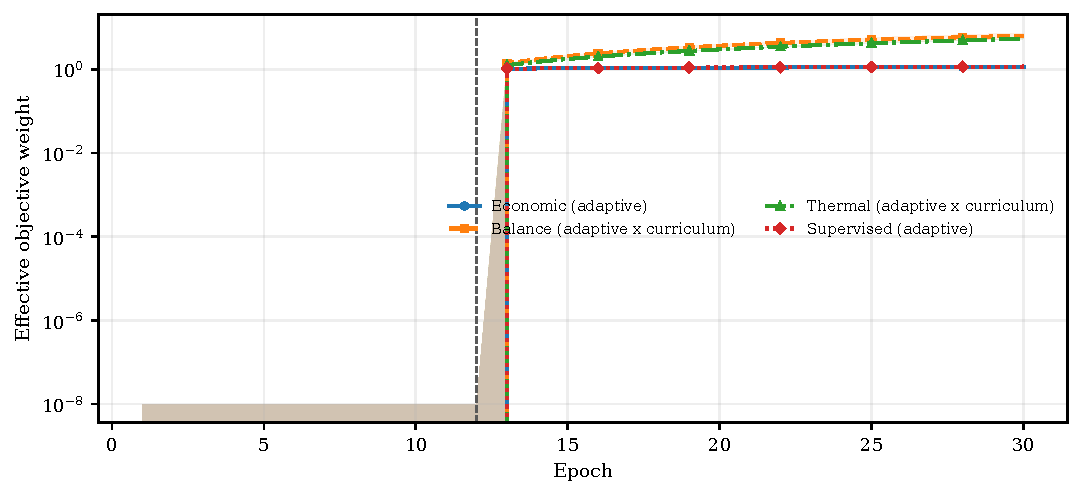
\includegraphics[width=\columnwidth]
    {figures/fig_adaptive_weights.pdf}
  \caption{IEEE 30 effective GFNO-PINO objective weights. Curves and shading are
  the five-seed mean and one standard deviation; balance and thermal curves
  include their curriculum multipliers. The angle loss remains below the
  $10^{-8}$ activation threshold under the nonrestrictive source bounds and
  therefore has zero active-set weight and is not shown.}
  \label{fig:adaptive_weights}
\end{figure}

Figures~\ref{fig:residual_convergence} and \ref{fig:adaptive_weights} expose
both training variance and the supervised-to-physics transition. Finite
weights verify numerical stability of the active-set scheme; they do not imply
convergence to the AC equality manifold. The complete per-epoch histories,
including raw losses, effective weights, and validation scores, are archived
for all 20 GFNO-PINO runs.

\subsection{Inference latency and scalability}

\begin{table*}[t]
\centering
\caption{Device-specific batch-one latency in milliseconds. Neural values are five-seed mean $\pm$ standard deviation of medians after warm-up; solver values are stored CPU medians. Preprocessing, transfer, verification, and restoration are excluded.}
\label{tab:latency}
\begin{tabular}{lrrrrr}
\toprule
System & IPOPT AC-OPF & DC-OPF & Topology-blind GFNO & Plain GNN & GFNO-PINO \\
\midrule
IEEE 30 & 57.29 & 25.52 & 5.56 $\pm$ 0.61 & 11.38 $\pm$ 0.60 & 6.94 $\pm$ 0.79 \\
IEEE 57 & 204.45 & 123.24 & 6.35 $\pm$ 0.50 & 14.23 $\pm$ 2.38 & 5.67 $\pm$ 0.25 \\
IEEE 118 & 524.17 & 155.79 & 5.54 $\pm$ 0.26 & 11.08 $\pm$ 1.07 & 6.19 $\pm$ 0.33 \\
IEEE 300 & 1484.22 & 191.22 & 9.13 $\pm$ 5.32 & 13.53 $\pm$ 0.36 & 10.75 $\pm$ 5.93 \\
\bottomrule
\end{tabular}
\end{table*}


The workstation contains a 13th-generation Intel Core i5-13420H CPU and an
NVIDIA GeForce RTX 3050 6 GB Laptop GPU. IPOPT and DC-OPF values are stored CPU
solver times; neural values are synchronized float32 CUDA forward-pass times
after warm-up. Table~\ref{tab:latency} is therefore a device-specific
comparison, not a hardware-matched solver acceleration. It excludes feature
construction, transfer, verification, and restoration. These omissions are
material because a prediction that fails the AC-feasibility proxy cannot
replace an AC-OPF solve without correction. GFNO-PINO's five-seed mean CUDA
medians are $6.94\pm0.79$, $5.67\pm0.25$, $6.19\pm0.33$, and
$10.75\pm5.93$ ms, whereas stored IPOPT CPU medians are 57.29, 204.45, 524.17,
and 1484.22 ms. The resulting raw ratios are 8.3, 36.1, 84.7, and 138.1;
they compare incomplete surrogate predictions with complete solver outputs,
not end-to-end feasible-solution speedups.

\begin{figure*}[t]
  \centering
  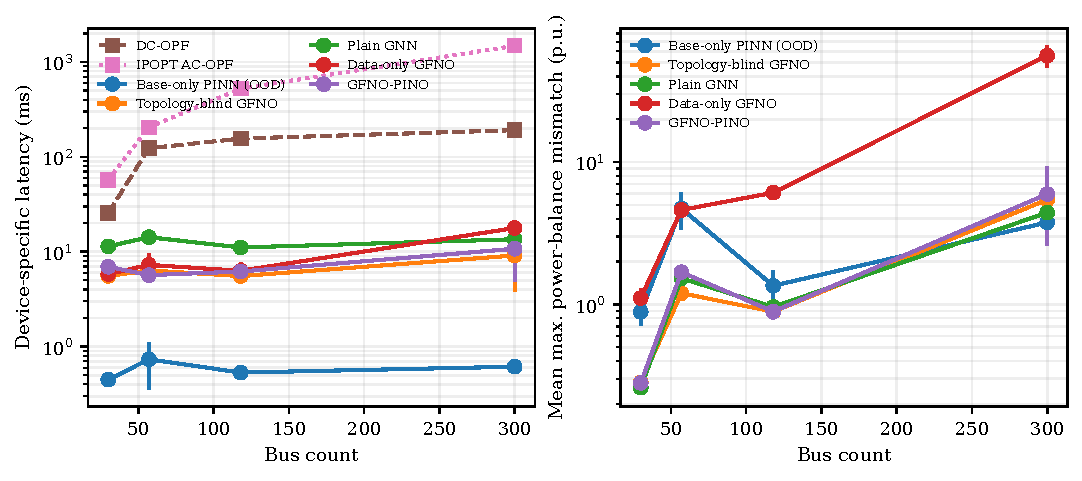
\includegraphics[width=0.90\textwidth]{figures/fig_scalability.pdf}
  \caption{Device-specific median batch-one latency and mean sample-maximum
  complex-power-balance mismatch versus bus count. Learned-model error bars
  are one standard deviation across five training seeds. Note: IEEE 57 and
  IEEE 300 use relaxed voltage bounds and IEEE 300 uses a reduced
  load-perturbation range relative to IEEE 30/118
  (Section~\ref{subsec:scenario_generation}); cross-system points therefore reflect
  differing electrical stress and should not be read as a controlled scaling
  sweep.}
  \label{fig:scalability}
\end{figure*}

\subsection{Unseen-topology generalization and ablation}
\label{subsec:ablation}

\begin{table*}[t]
\centering
\caption{Four-system, five-seed ablation averages. Mismatch and thermal-excess magnitudes are p.u. Voltage, generator, and angle violation rates and excesses are zero for every method.}
\label{tab:generalization}
\resizebox{\textwidth}{!}{%
\begin{tabular}{lcccrrrrrr}
\toprule
Model & Topol. input & Spectral & Physics & $|\Delta C_{\rm ref}|$ (\%) & Mean bus & Mean max. & Therm. rate (\%) & Therm. max. & AC feas. (\%) \\
\midrule
Base-only PINN (OOD) & Base only & No & Yes & 15.0 & 0.546 & 2.681 & 2.98 & 1.39e-01 & 0.0 \\
Topology-blind GFNO & No & Yes & Yes & 26.8 & 0.365 & 1.952 & 0.25 & 5.15e-03 & 0.0 \\
Plain GNN & Yes & No & Yes & 21.9 & 0.372 & 1.790 & 0.25 & 1.74e-03 & 0.0 \\
Data-only GFNO & Yes & Yes & No & 10.9 & 1.534 & 16.951 & 1.63 & 1.99e-01 & 0.0 \\
GFNO-PINO & Yes & Yes & Yes & 27.6 & 0.378 & 2.204 & 0.25 & 2.15e-03 & 0.0 \\
\bottomrule
\end{tabular}
}
\end{table*}


Table~\ref{tab:generalization} separates three questions. The matched
topology-blind GFNO tests whether the explicit topology field is useful when
the training rows are held constant. The plain GNN tests Chebyshev spectral
propagation against spatial aggregation. The data-only GFNO tests the effect of
physics fine-tuning. Results are averaged first within each case and seed and
then across the four cases, so a large system does not dominate by bus count.
The base-only PINN is shown as an OOD operational reference but is not used as
the causal topology ablation. Five-seed dispersion is supplied in the
case-level CSVs; the benchmark supports only effects that remain visible
relative to that dispersion.

The observed physics-fine-tuning effect is positive under this pilot protocol,
but the architectural conclusions are negative. Averaged across systems, mean
sample-maximum mismatch falls from 16.951 p.u. for the data-only GFNO to
2.204 p.u. for GFNO-PINO. In contrast, the matched topology-blind GFNO averages
1.952 p.u. and is better on IEEE 57, 118, and 300; GFNO-PINO is only 0.7\%
lower on IEEE 30. Thus, these experiments
do not demonstrate a causal accuracy benefit from the explicit topology field.
The spatial GNN averages 1.790 p.u. and is better than GFNO-PINO on three of
four systems, so a Chebyshev advantage is likewise not established. These
outcomes do not invalidate the directional topology-conditioned formulation;
they show that the present data volume, loss, and training budget are
insufficient to validate its claimed architectural advantage.
Table~\ref{tab:generalization} includes all declared aggregate physical
diagnostics for every learned method. Case-level values, P95 and worst balance
mismatch, signed reference-cost differences, label errors, and
topology-resolved values remain
available in the accompanying CSVs rather than being collapsed into a visually
unreadable manuscript table.

\section{Limitations}
\label{sec:limitations}

The bounded output layer guarantees independent voltage and generator bounds
and the reference angle, but it does not project onto the full non-convex AC
feasible set. Complex-power balance, thermal loading, and branch
angle-difference limits are soft objectives; any deployment
requires explicit verification and an AC correction solve. Satisfaction of
one inequality class cannot repair equality infeasibility. Although the
benchmark now uses five seeds, it still uses only 12 selected topology IDs per
system, synthetic renewable profiles, and 30 training epochs. It is therefore
a controlled outage-generalization study rather than full security-constrained
coverage. The deterministic first-eligible selection was not stratified by
loading severity, voltage sensitivity, or electrical distance, and severity
descriptors for the unselected eligible outages were not generated. Results
therefore must not be read as representative of the complete N-1 set.
Moreover, the matched topology-blind GFNO and spatial GNN have lower
four-system mean maximum balance mismatch than GFNO-PINO. The experiment
therefore demonstrates that the implementation can consume unseen topology
fields, but not that those fields or the Chebyshev layer improve accuracy under
the present protocol.

The method is evaluated only through 300 buses, and the current dense Laplacian
batching path is not evidence of scalability to substantially larger
interconnections. Although the parameterization is node- and edge-based, the
experiments use one checkpoint per grid size; they do not demonstrate one
shared checkpoint across 30--300 buses. Generalization is limited to
non-islanding single-line outages within a fixed network family and does
not cover bus additions, generator-set changes, islands, or simultaneous N-k
contingencies. The relaxed IEEE 57/300 voltage ranges and reduced IEEE 300 load
range further limit direct cross-case stress comparisons. Finally, IPOPT
provides locally converged references rather than global-optimality
certificates, and the rejected scenarios---particularly the 154 IEEE 30
failures---may introduce selection bias.

Finally, the localized Chebyshev polynomial is structurally a ChebNet graph
convolution. No mesh-refinement, discretization-transfer, or shared
mixed-size-checkpoint experiment was performed. Consequently, this paper uses
``GFNO-PINO'' only as the archived model identifier and does not claim a
neural-operator property beyond topology-conditioned finite-graph prediction.

\section{Conclusion}
\label{sec:conclusion}

The central finding of this controlled ablation is that physics-informed
fine-tuning is the only tested design choice with a consistent improvement
under the pilot protocol; benefits from explicit topology conditioning and
Chebyshev spectral filtering are not confirmed. The topology-conditioned
GFNO-PINO model is therefore an instrument for separating these effects, not a
demonstrated superior architecture. Its Chebyshev polynomial filter of the
sample-specific normalized Laplacian preserves a graph
spectral inductive bias without requiring eigenvector alignment after line
outages. Explicit branch status and admittance features make contingencies
predictor inputs, while exact $Y$, $Y_f$, and $Y_t$ matrices define
differentiable AC residuals. Bounded output transformations enforce voltage
and generator boxes and the slack reference; they are deliberately not
presented as a complete AC-feasibility guarantee.

The executed benchmark uses 564 locally converged IPOPT labels and 3600
held-out neural evaluations spanning four systems, five model variants, and
five training seeds. Under this pilot protocol, paired physics fine-tuning
runs reduce mean sample-maximum balance mismatch by 63.4--89.3\% relative to
the data-only GFNO; all 20 observed paired seed effects are positive, while
the descriptive resampling intervals are not population-confidence claims.
Nevertheless, GFNO-PINO retains 0.281--5.959 p.u. mean maximum mismatch, has a
1.0\% thermal-violation rate on IEEE 30, and produces no prediction
meeting the declared AC-feasibility proxy. Its four-system balance average
(2.204 p.u.) is also worse than the matched topology-blind GFNO (1.952 p.u.)
and spatial GNN (1.790 p.u.), so neither a topology-input nor a Chebyshev
advantage is supported. CUDA forward-pass medians yield raw device-specific
latency ratios (speedups) of 8.3--138.1$\times$ relative to stored IPOPT CPU
solve medians, but that comparison excludes the correction
required for feasibility. Signed negative reference-cost differences are
therefore infeasible lower-cost points, not optimality gains.

The defensible role of the present model is a topology-conditioned research
prototype for warm starts or screening whose output is independently checked,
not a stand-alone certified AC-OPF solver. The negative ablations are
scientifically important: representational access to topology is necessary for
the intended surrogate, but this benchmark does not show that the network learns
to exploit it better than simpler alternatives.

The next step is an explicit differentiable feasibility-restoration layer or
post-network Newton/AC-OPF correction, followed by full N-1 coverage, real
renewable time series, sparse mixed-size batching, and hardware-matched
end-to-end latency accounting. N-k, island-aware operation, uncertainty
quantification, and validation on operational networks remain open. Until
those steps produce verified feasible outputs, independent solver validation
is necessary for safety-critical dispatch.

\section*{Data and code availability}

The accompanying archive contains the implementation, locked environments,
configuration and data-generation files, exact topology and constraint
manifests, solver-labelled pilot data, every case--model--seed checkpoint and
history, per-sample evaluations, aggregate CSV files, tests, and the scripts
that regenerate all tables and figures. A SHA-256 manifest covers the released
artifacts, and the README gives a single reproduction command. Source
IEEE/MATPOWER cases remain subject to their upstream licenses. The submitted
supplement is named
\path{topology_conditioned_gfno_pino_submission.zip}; its companion
\path{topology_conditioned_gfno_pino_submission.sha256.json} provides
the transport checksum. A permanent public
repository DOI has not yet been assigned and must be supplied by the authors
or journal repository before publication; this manuscript does not invent a
locator that was unavailable at revision time.

\bibliographystyle{elsarticle-num}
\bibliography{references}

\end{document}
